\documentclass[]{beamer}
\usepackage{etex}
\usepackage{fancyvrb}
\usepackage{tikz}
\usetikzlibrary{arrows}
\tikzset{>=latex}

\newcommand{\myref}[1]{\small\item\url{#1}}
\newcommand{\myreff}[1]{\scriptsize\item\url{#1}}

\newcommand{\mthree}[9]{
\left[
\begin{array}{ccc}
#1 & #2 & #3 \\ #4 & #5 & #6 \\ #7 & #8 & #9
\end{array}
\right]
}

\newcommand{\mrowsix}[6]{
#1 & #2 & #3 & #4 & #5 & #6 
}

\newcommand{\bi}{\begin{itemize}}
\newcommand{\ei}{\end{itemize}}
\newcommand{\sect}[1]{
\section{#1}
\begin{frame}[fragile]\frametitle{#1}
}


\newcommand{\myvec}[1]{
\pstThreeDDot[showpoints=true,drawCoor=true](#1)
\pstThreeDLine[arrows=->,linecolor=blue](0,0,0)(#1)
}


\mode<presentation>
{
%  \usetheme{Madrid}
  % or ...

%  \setbeamercovered{transparent}
  % or whatever (possibly just delete it)
}

\usepackage[english]{babel}

\usepackage[latin1]{inputenc}

\title[Linear Algebra Notes II]
{
Linear Algebra Notes
}

%\subtitle{Based on Slides in MIT Open Courseware} % (optional)

\author[Geoffrey Matthews]
{Geoffrey Matthews}
% - Use the \inst{?} command only if the authors have different
%   affiliation.

\institute[WWU/CS]
{
  Department of Computer Science\\
  Western Washington University
}
% - Use the \inst command only if there are several affiliations.
% - Keep it simple, no one is interested in your street address.

\date{Fall 2011}

% If you have a file called "university-logo-filename.xxx", where xxx
% is a graphic format that can be processed by latex or pdflatex,
% resp., then you can add a logo as follows:

%\pgfdeclareimage[height=0.5cm]{university-logo}{WWULogoProColor}
%\logo{\pgfuseimage{university-logo}}

% If you wish to uncover everything in a step-wise fashion, uncomment
% the following command: 

%\beamerdefaultoverlayspecification{<+->}
\newcommand{\point}[2]{
  \fill (#1) node (#2) {} circle (2pt) node[anchor=south] {$#2$};
  }
\newcommand{\pointn}[2]{
  \fill (#1) node (#2) {} circle (2pt) node[anchor=north] {$#2$};
}
\newcommand{\pointnw}[2]{
  \fill (#1) node (#2) {} circle (2pt) node[anchor=north west] {$#2$};
  }
\newcommand{\coords}{
      \draw[dotted,step=1] (0,0) grid (9.9,9.9);
      \draw[thick,<->] (10,0) %node[anchor=west] {$x$ axis}
      -- (0,0) -- (0,10) %node[anchor=south] {$y$ axis}
      ;
      \foreach \x in {0,1,2,3,4,5,6,7,8,9}
        \draw (\x ,2pt) -- (\x ,-2pt) node[anchor=north] {$\x$};
      \foreach \y in {0,1,2,3,4,5,6,7,8,9}
        \draw (2pt,\y) -- (-2pt,\y ) node[anchor=east] {$\y$};
}

\begin{document}


\begin{frame}
  \titlepage
\end{frame}

%\begin{frame}
%  \frametitle{Outline}
%  \tableofcontents
%  % You might wish to add the option [pausesections]
%\end{frame}


\sect{Online Resources}

{\bf Readings}
\begin{itemize}
  \myref{http://chortle.ccsu.edu/vectorlessons/vectorindex.html}
  \myref{http://mathforum.org/mathimages/index.php/Math_for_Computer_Graphics_and_Computer_Vision}
\myref{http://cs229.stanford.edu/section/cs229-linalg.pdf}

\myreff{http://ocw.mit.edu/courses/electrical-engineering-and-computer-science/}, Computer graphics
\myref{http://joshua.smcvt.edu/linearalgebra/}
\end{itemize}
{\bf Videos}
\begin{itemize}
\myref{http://www.khanacademy.org/math/linear-algebra}
\end{itemize}
\end{frame}

\sect{Points in space}
\begin{columns}[onlytextwidth]
\begin{column}{0.6\textwidth}
  \tikzset{>=latex,x=0.6cm,y=0.6cm}
  \begin{tikzpicture}
    \coords
    \point{3,7}{p}
    \point{9,3}{q}
    \point{2,5}{r}
    \point{4,1}{s}
    \point{8,6}{t}
  \end{tikzpicture}
\end{column}
\begin{column}{0.4\textwidth}
  \begin{itemize}
  \item Points exist in space without a coordinate system.
  \item We introduce coordinates to make it easier to compute with them.
  \item But the coordinates are arbitrary, so long as they're consistent.
  \end{itemize}
  \end{column}
\end{columns}
\end{frame}


\sect{Vectors}
\begin{columns}[onlytextwidth]
\begin{column}{0.6\textwidth}
  \tikzset{>=latex,x=0.6cm,y=0.6cm}
  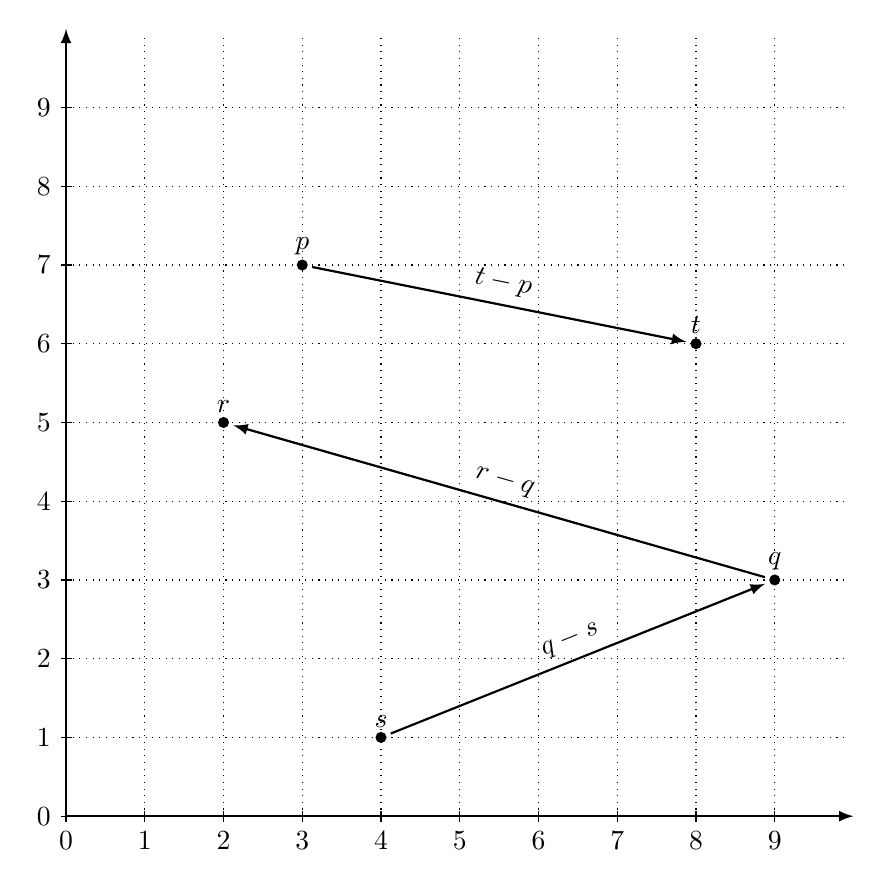
\begin{tikzpicture}
    \coords
    \point{3,7}{p}
    \point{9,3}{q}
    \point{2,5}{r}
    \point{4,1}{s}
    \point{8,6}{t}
    \draw[thick,->] (p) -- (t) node[midway,anchor=south,sloped] {$t-p$};
    \draw[thick,->] (q) -- (r) node[midway,anchor=south,sloped] {$r-q$};
    \draw[thick,->] (s) -- (q) node[midway,anchor=south,sloped] {$q-s$};
  \end{tikzpicture}
\end{column}
\begin{column}{0.4\textwidth}
  \begin{itemize}
  \item Subtracting two points results in a vector.
\item Both points and vectors in $n$ dimensions are represented by $n$
  real numbers. 
  \end{itemize}
  \end{column}
\end{columns}
\end{frame}

\sect{Points {\em vs.} Vectors}
\begin{columns}[onlytextwidth]
\begin{column}{0.6\textwidth}
  \tikzset{>=latex,x=0.6cm,y=0.6cm}
  \begin{tikzpicture}
    \coords
    \point{3,7}{p}
    \point{9,3}{q}
    \point{2,5}{r}
    \point{4,1}{s}
    \point{8,6}{t}
    \draw[thick,->] (p) -- (t) node[midway,anchor=south,sloped] {$u$};
    \draw[thick,->] (q) -- (r) node[midway,anchor=south,sloped] {$v$};
    \draw[thick,->] (s) -- (q) node[midway,anchor=south,sloped] {$w$};
  \end{tikzpicture}
\end{column}
\begin{column}{0.4\textwidth}
  \begin{itemize}
  \item A point is a position.
  \item A vector is a magnitude and a direction.
  \end{itemize}
  \end{column}
\end{columns}
\end{frame}

\sect{Vector Addition}
\begin{columns}[onlytextwidth]
\begin{column}{0.6\textwidth}
  \tikzset{>=latex,x=0.6cm,y=0.6cm}
  \begin{tikzpicture}
    \coords
    \point{3,7}{p}
    \point{9,3}{q}
    \point{2,5}{r}
    \point{4,1}{s}
    \point{8,6}{t}
    \draw[thick,->] (s) -- (r) node[midway,anchor=south,sloped] {$u$};
    \draw[thick,->] (r) -- (t) node[midway,anchor=south,sloped] {$v$};
    \draw[thick,->] (s) -- (t) node[midway,anchor=south,sloped] {$w$};
  \end{tikzpicture}
\end{column}
\begin{column}{0.4\textwidth}
  \begin{eqnarray*}
    u &=& r-s\\
    v &=& t-r\\
    w &=& t-s\\
    w &=& u + v\\
    r &=& s + u\\
    t &=& r + v\\
   t &=& s + w
  \end{eqnarray*}
  \hfill
  You can't add points!
  \end{column}
\end{columns}
\end{frame}

\sect{Vectors do not have positions}
\begin{columns}[onlytextwidth]
\begin{column}{0.6\textwidth}
  \tikzset{>=latex,x=0.6cm,y=0.6cm}
  \begin{tikzpicture}
    \coords
    \draw[thick,->] (1,1) -- (3,5) node[midway,anchor=south,sloped] {$u$};
    \draw[thick,->] (5,2) -- (7,6) node[midway,anchor=south,sloped] {$v$};
    \draw[thick,->] (3,6) -- (5,10) node[midway,anchor=south,sloped] {$w$};
  \end{tikzpicture}
\end{column}
\begin{column}{0.4\textwidth}
  \begin{itemize}
  \item These are all the same vector
    \item $u=v=w$
    \end{itemize}
  \end{column}
\end{columns}
\end{frame}

\sect{Vectors multiplied by scalars}
\begin{columns}[onlytextwidth]
\begin{column}{0.6\textwidth}
  \tikzset{>=latex,x=0.6cm,y=0.6cm}
  \begin{tikzpicture}
    \coords
    \draw[thick,->] (2,8) -- (4,9) node[midway,anchor=south,sloped] {$v$};
    \draw[thick,->] (2,6) -- (6,8) node[midway,anchor=south,sloped] {$2v$};
    \draw[thick,->] (2,4) -- (8,7) node[midway,anchor=south,sloped] {$3v$};
    \draw[thick,->] (5,3) -- (3,2) node[midway,anchor=south,sloped] {$-v$};
  \end{tikzpicture}
\end{column}
\begin{column}{0.4\textwidth}
  \begin{itemize}
  \item Multiplication is repeated addition.
    \end{itemize}
  \end{column}
\end{columns}
\end{frame}


\sect{Lines defined by point and vector}
\begin{columns}[onlytextwidth]
\begin{column}{0.6\textwidth}
  \tikzset{>=latex,x=0.6cm,y=0.6cm}
  \begin{tikzpicture}
    \coords
    \point{1,5}{p}
    \point{7,5.75}{p+xv}
    \draw[thick,->] (p) -- (3,5.25) node[midway,anchor=south,sloped] {$v$};
    \draw[dashed] (-1,4.75) -- (11,6.25);
  \end{tikzpicture}
\end{column}
\begin{column}{0.4\textwidth}
  \begin{itemize}
  \item The line through $p$ in the direction $v$ is the set of all
    points $p + xv$ for some $x\in\mathbb{R}$
    \end{itemize}

  \end{column}
\end{columns}
\end{frame}




\sect{Planes defined by point and two vectors}
\begin{columns}[onlytextwidth]
\begin{column}{0.6\textwidth}
  \tikzset{>=latex,x=0.6cm,y=0.6cm}
  \begin{tikzpicture}
    \coords
    \pointnw{2,2}{p}
    \point{6,8}{p+xv + yw}
    \draw[thick,->] (p) -- (4,3) node[midway,anchor=south,sloped] {$v$};
    \draw[thick,->] (p) -- (2,4) node[midway,anchor=south,sloped] {$w$};
    \draw[dashed] (-1,0.5) -- (10,6);
    \draw[dashed] (2,-1) -- (2,10);
    \draw[dashed] (6,4) -- (6,8);
    \draw[dashed] (2,6) -- (6,8);
  \end{tikzpicture}
\end{column}
\begin{column}{0.4\textwidth}
  \begin{itemize}
  \item The plane through $p$ aligned with $v$ and $w$ is the set of all
    points $p + xv + yw$ for some $x,y\in\mathbb{R}$
    \end{itemize}

  \end{column}
\end{columns}
\end{frame}

\sect{Frames}
\begin{columns}[onlytextwidth]
\begin{column}{0.6\textwidth}
  \tikzset{>=latex,x=0.6cm,y=0.6cm}
  \begin{tikzpicture}
    \coords
    \point{7,8}{q}
    \pointn{3,2}{p}
    \draw[thick,->,red] (p) -- (5,2) node[anchor=west] {$v$};
    \draw[thick,->,blue] (p) -- (3,3) node[anchor=south] {$w$};
  \end{tikzpicture}
\end{column}
\begin{column}{0.4\textwidth}

  \begin{itemize}
  \item A tuple consisting of a point (the origin) and
    $n$ vectors is a {\em frame}.
  \end{itemize}
\[f = \langle p,v,w\rangle\]
\begin{itemize}
\item A frame gives coordinates to points.
\item $q = p + 2v + 6w$
  \item $q = (2,6)_f$

  \end{itemize}
  \end{column}
\end{columns}
\vfill

An {\em orthonormal} frame is one in which all the vectors are
  unit length and perpendicular to each other.
\end{frame}


\sect{Affine sums of vectors}
\begin{columns}[onlytextwidth]
\begin{column}{0.6\textwidth}
  \tikzset{>=latex,x=0.6cm,y=0.6cm}
  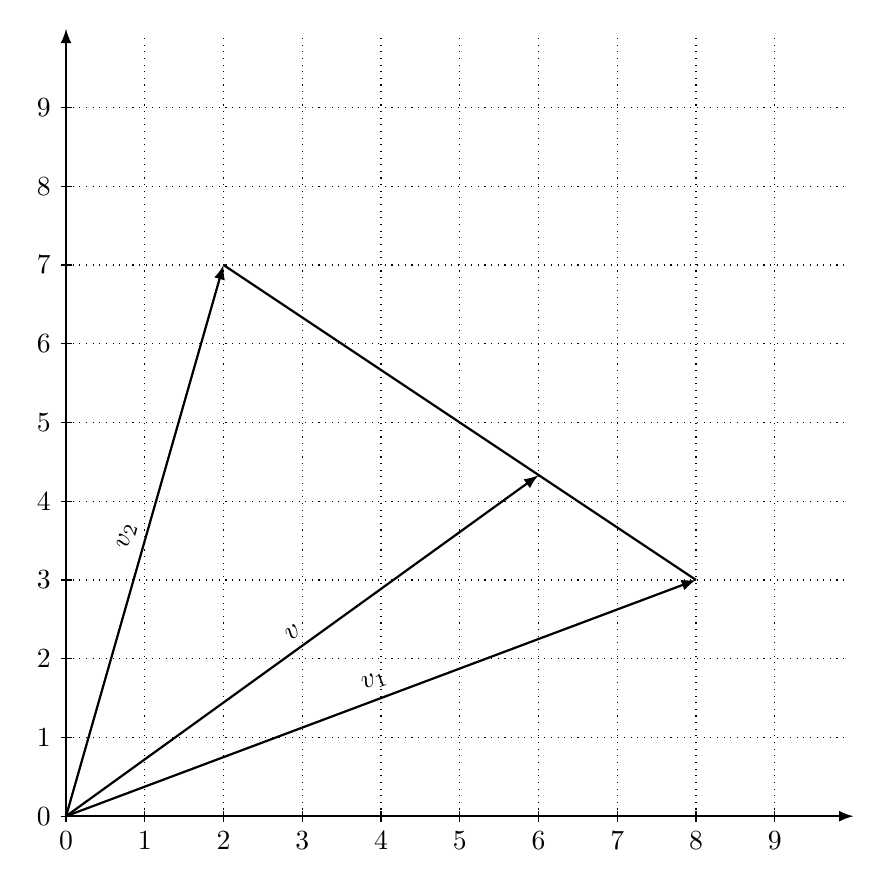
\begin{tikzpicture}
    \coords
    \draw[thick,->] (0,0) -- (8,3) node[midway,anchor=south,sloped] {$v_1$};
    \draw[thick,->] (0,0) -- (2,7) node[midway,anchor=south,sloped] {$v_2$};
    \draw[thick,->] (0,0) -- (6,4.33) node[midway,anchor=south,sloped] {$v$};
    \draw[thick,-] (8,3) -- (2,7);
  \end{tikzpicture}
\end{column}
\begin{column}{0.4\textwidth}
\[ 0 \leq a \leq 1\]
  \begin{eqnarray*}
    v &=& (1-a)v_1 + av_2\\
    &=& v_1 + a(v_2-v_1)
  \end{eqnarray*}
  Or:
  

  \begin{eqnarray*}
&&   0 \leq a_i \leq 1\\
    1 &=& a_1 + a_2 \\
    v &=& a_1v_1 + a_2 v_2
    \end{eqnarray*}
  \end{column}
\end{columns}
\end{frame}



\sect{Affine sums of vectors}
\begin{columns}[onlytextwidth]
\begin{column}{0.6\textwidth}
  \tikzset{>=latex,x=0.6cm,y=0.6cm}
  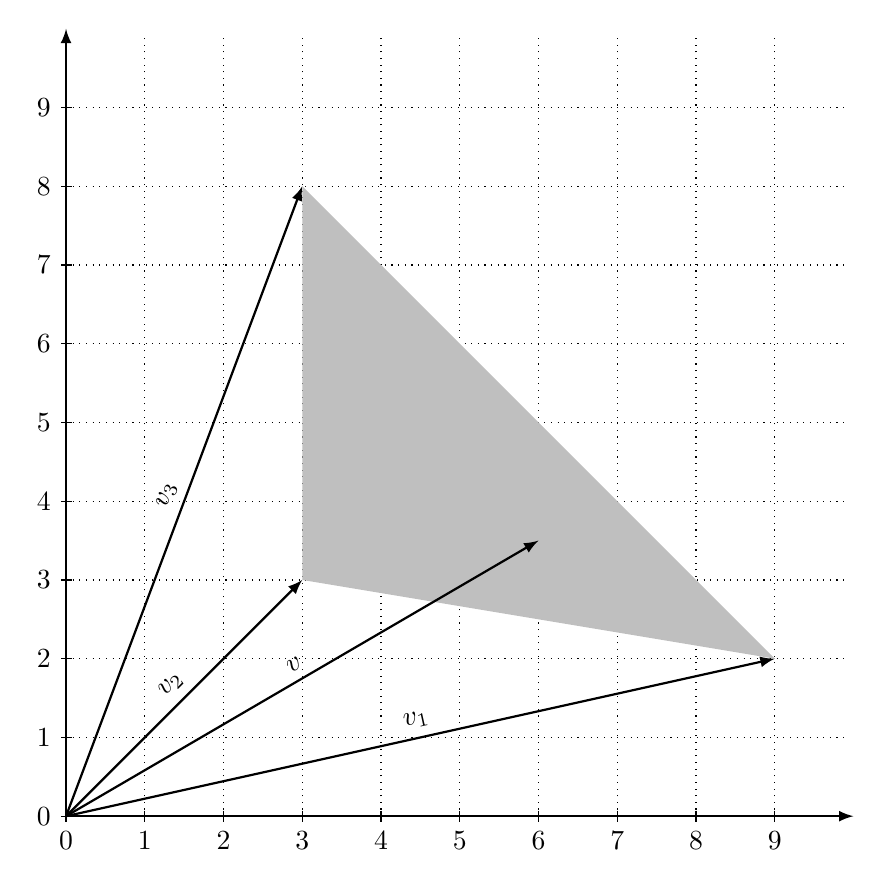
\begin{tikzpicture}
    \coords
    \draw[thick,->] (0,0) -- (9,2) node[midway,anchor=south,sloped] {$v_1$};
    \draw[thick,->] (0,0) -- (3,3) node[midway,anchor=south,sloped] {$v_2$};
    \draw[thick,->] (0,0) -- (3,8) node[midway,anchor=south,sloped] {$v_3$};
    \path[fill=lightgray] (9,2) -- (3,3) -- (3,8);
    \draw[thick,->] (0,0) -- (6,3.5) node[midway,anchor=south,sloped] {$v$};
  \end{tikzpicture}
\end{column}
\begin{column}{0.4\textwidth}

\begin{eqnarray*}
&& 0 \leq a_i \leq 1\\
  1 &=& a_1 + a_2 + a_3 \\
    v &=& a_1v_1 + a_2v_2 + a_3v_3
  \end{eqnarray*}

  \end{column}
\end{columns}
\end{frame}


\sect{Trigonometry}
\begin{columns}[onlytextwidth]
\begin{column}{0.6\textwidth}
  \tikzset{>=latex,x=5cm,y=5cm}
  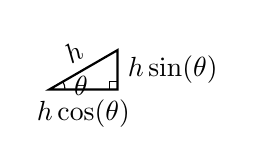
\begin{tikzpicture}
    \draw[thick] (0,0)
    -- (0.866,0) node[midway,anchor=north] {$h\cos(\theta)$}
    -- (0.866,0.5) node[midway,anchor=west] {$h\sin(\theta)$}
    -- cycle node[midway,anchor=south,sloped] {$h$};
    \draw (.2,0) arc (0:30:.2)  node[midway,anchor=west] {$\theta$};
    \draw[thin] (0.766,0.0) -- (.766,0.1) --  (.866,0.1);
  \end{tikzpicture}
\end{column}
\begin{column}{0.4\textwidth}

\begin{eqnarray*}
  \tan(\theta) &=& \frac{\sin(\theta)}{\cos(\theta)}\\
  &=& \frac{1}{\cot(\theta)}\\
  \sin(\theta) &=& \frac{1}{\csc(\theta)}\\
  \cos(\theta) &=& \frac{1}{\sec(\theta)}\\
  \end{eqnarray*}

  \end{column}
\end{columns}
\end{frame}


\sect{More Trigonometry}
  \tikzset{>=latex,x=3cm,y=3cm}
  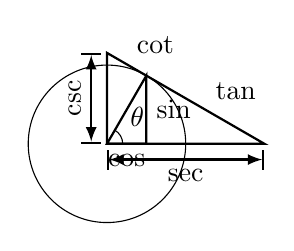
\begin{tikzpicture}
    \draw[thick] (0,0)
    -- (0.5,0) node[midway,anchor=north] {cos}
    -- (0.5,0.866) node[midway,anchor=west] {sin}
    -- cycle;
    \draw (.2,0) arc (0:60:.2)  node[midway,anchor=south west] {$\theta$};
    \draw (0,0) circle (1);
    \draw[thick] (0,0)
    -- (2,0)
    -- (0.5,0.866) node [midway,anchor=south west] {tan}
    -- (0,1.155) node [midway,anchor=south west] {cot}
    -- cycle;
    \draw[|<->|,thick] (0,-.2)
    -- (2,-.2) node[midway,anchor=north,sloped] {sec};
    \draw[|<->|,thick] (-.2,0)
    -- (-.2,1.155) node[midway,anchor=south,sloped] {csc};
  \end{tikzpicture}

\end{frame}

\sect{Dot product}
\begin{columns}[onlytextwidth]
\begin{column}{0.6\textwidth}
  \tikzset{>=latex,x=.6cm,y=.6cm}
  \begin{tikzpicture}
    \draw[thick,->] (0,0) -- (8,0) node[midway,anchor=south]{$u$};
    \draw[thick,->] (0,0) -- (5,5) node[midway,anchor=south]{$v$};
    \draw (1,0) arc (0:45:1)  node[midway,anchor=west] {$\theta$};
  \end{tikzpicture}
\end{column}
\begin{column}{0.4\textwidth}
  In 2D
  \begin{eqnarray*}
    u\cdot v &=& \cos(\theta)|u||v|\\
    &=& u_xv_x + u_yv_y
  \end{eqnarray*}
  In 3D
  \begin{eqnarray*}
    u\cdot v &=& \cos(\theta)|u||v|\\
    &=& u_xv_x + u_yv_y + u_zv_z
  \end{eqnarray*} 
  Note:
  \begin{eqnarray*}
    u\cdot u &=& \cos(\theta)|u||u|\\
    &=& u_xu_x + u_yu_y + u_zu_z\\
    &=& |u|^2
  \end{eqnarray*}
  
\end{column}

\end{columns}
\end{frame}

\sect{Projection of one vector on another}
\begin{columns}[onlytextwidth]
  \begin{column}{0.6\textwidth}
    \tikzset{>=latex,x=.6cm,y=.6cm}
    \begin{tikzpicture}
      \draw[thick,->] (0,0) -- (8,0) node[anchor=south]{$u$};
      \draw[thick,->] (0,0) -- (5,5) node[midway,anchor=south]{$v$};
      \draw (1,0) arc (0:45:1)  node[midway,anchor=west] {$\theta$};
      \draw[dashed] (5,0) -- (5,5);
      \draw[|<->|] (0,-0.5) -- (5,-0.5) node[midway,anchor=north] {$x$};
    \end{tikzpicture}
  \end{column}
  \begin{column}{0.4\textwidth}
    \begin{itemize}
    \item What is $x$?\pause
    \end{itemize}
    \begin{eqnarray*}
    x &=& \cos(\theta)|v|\\\\\pause
    v\cdot u &=& \cos(\theta)|u||v|\\\\
    \cos(\theta) &=& \frac{u\cdot v}{|u||v|}\\\\
    x &=& \frac{u\cdot v}{|u|}
    \end{eqnarray*}
    \end{column}
  \end{columns}
\end{frame}

\sect{Same direction, opposite direction}
\begin{columns}[onlytextwidth]
  \begin{column}{0.6\textwidth}
    \tikzset{>=latex,x=.6cm,y=.6cm}
    \begin{tikzpicture}
      \draw[thick,->] (0,0) -- (8,0) node[anchor=south]{$u$};
      \draw[thick,->] (0,0) -- (5,3) node[anchor=south]{$v_1$};
      \draw[thick,->] (0,0) -- (0,4) node[anchor=south]{$v_2$};
      \draw[thick,->] (0,0) -- (-2,3) node[anchor=south]{$v_3$};
    \end{tikzpicture}
  \end{column}
  \begin{column}{0.4\textwidth}
    \begin{itemize}
    \item What is the sign of $u\cdot v_i$?
    \end{itemize}
    \end{column}
  \end{columns}
\end{frame}


\sect{{\em AMAZING} theorem about the dot product.}
\begin{itemize}
\item In any coordinate system whatsoever:
\begin{eqnarray*}
u\cdot v &=& (u_x, u_y, u_z)\cdot (v_x, v_y, v_z) \\
&=& u_xv_x + u_yv_y + u_zv_z\\
&=& [u_x\  u_y\  u_z]\left[\begin{array}{c}v_x\\v_y\\v_z\end{array}\right]\\
&=& u^Tv
\end{eqnarray*}
\end{itemize}

\end{frame}

\sect{Example use of dot product:  reflected ray}
\begin{columns}
  \begin{column}{0.6\textwidth}
    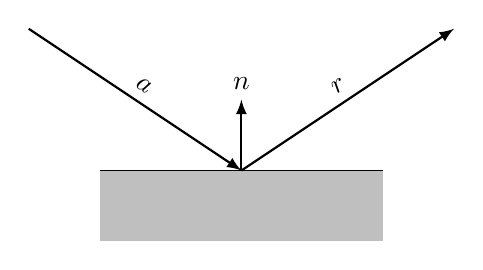
\begin{tikzpicture}[x=.9cm,y=.9cm]
      \fill[lightgray] (-2,0) -- (2,0) -- (2,-1) -- (-2, -1) -- cycle;
      \draw (-2,0) -- (2,0) ;
      \draw[thick,->] (-3,2) -- (0,0) node[midway,anchor=south,sloped] {$a$};
      \draw[thick,->] (0,0) -- (0,1) node[anchor=south] {$n$};
      \draw[thick,->] (0,0) -- (3,2) node[midway,anchor=south,sloped] {$r$};
    \end{tikzpicture}
  \end{column}
  \begin{column}{0.4\textwidth}
    \begin{itemize}
    \item How do we reflect ray $a$ about normal $n$ to get $r$?
    \end{itemize}
  \end{column}
\end{columns}

\end{frame}

\sect{Reflected ray}
\begin{columns}
  \begin{column}{0.6\textwidth}
    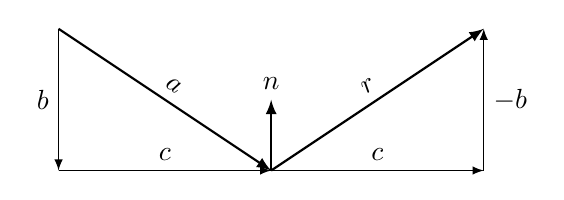
\begin{tikzpicture}[x=.9cm,y=.9cm]
      \draw[thick,->] (-3,2) -- (0,0) node[midway,anchor=south,sloped] {$a$};
      \draw[thick,->] (0,0) -- (0,1) node[anchor=south] {$n$};
      \draw[thick,->] (0,0) -- (3,2) node[midway,anchor=south,sloped] {$r$};
      \draw[->] (-3,2) -- (-3,0) node[midway,anchor=east] {$b$};
      \draw[->] (-3,0) -- (0,0) node[midway,anchor=south] {$c$};
      \draw[->] (0,0) -- (3,0) node[midway,anchor=south] {$c$};
      \draw[->] (3,0) -- (3,2) node[midway,anchor=west] {$-b$};
    \end{tikzpicture}
  \end{column}
  \begin{column}{0.4\textwidth}
    \begin{eqnarray*}
      a &=& b+c\\
      r &=& -b+c
    \end{eqnarray*}
    How do we find $b$ and $c$?
    \pause
      Assume $|n| = 1$
    \begin{eqnarray*}
      b &=& (a\cdot n)n\\
      c &=& a - b
    \end{eqnarray*}
    What if $|n|\not = 1$?
    \pause
    \begin{eqnarray*}
      b &=& \frac{(a\cdot n)}{(n\cdot n)}n\\
    \end{eqnarray*}
    
  \end{column}
\end{columns}

\end{frame}

\sect{Example use of the dot product}
\begin{center}
\begin{tikzpicture}
%\draw[help lines] (0,0) grid (8,4);
\draw[thick,*-*] (0,0) node [left] {$q$} -- (8,4) node [right] {$r$};
\draw[thick,*-*] (1,3)  node [left] {$p$};
\draw[thick,dashed,red] (1,3) -- (2,1) node[midway,above] {$x$};
\end{tikzpicture}
\end{center}
\bi
\item An object at $p$ is approaching a wall determined by points $q$ and $r$.
  \item How far away is the wall?
\ei
\end{frame}

\sect{How far away is the wall?}
\begin{center}
\begin{tikzpicture}
%\draw[help lines] (0,0) grid (8,4);
\draw[thick,->] (0,0) node [left] {$q$} -- (8,4) node [right] {$r$} node [midway,below] {$u$};
\draw[thick,->] (0,0)  -- (1,3) node [left] {$p$} node [midway,left] {$v$};
\draw[thick,dashed,red] (1,3) -- (2,1) node [midway,above] {$x$};
\end{tikzpicture}
\end{center}
\bi
\item Let's get some vectors:
  \begin{eqnarray*}
    v &=& p-q\\ u &=& r-q 
\end{eqnarray*}
\item Now what?
\ei
\end{frame}

\sect{How far away is the wall?}
\begin{center}
\begin{tikzpicture}
%\draw[help lines] (0,0) grid (8,4);
\draw[thick,->] (0,0) node [left] {$q$} -- (8,4) node [right] {$r$} node [midway,below] {$u$};
\draw[thick,->] (0,0)  -- (1,3) node [left] {$p$} node [midway,left] {$v$};
\draw[thick,dashed,red] (1,3) -- (2,1) node [midway,above] {$x$};
\draw[thick,dashed,red,xshift=.25em,yshift=-.5em,|-|] (0,0) -- (2,1) node [midway,below] {$y$};
\end{tikzpicture}
\end{center}
\bi
\item Can we find $y$?
\item Will that give us $x$?
\ei
\end{frame}

\sect{How far away is the wall?}
\begin{center}
\begin{tikzpicture}
%\draw[help lines] (0,0) grid (8,4);
\draw[thick,->] (0,0) node [left] {$q$} -- (8,4) node [right] {$r$} node [midway,below] {$u$};
\draw[thick,->] (0,0)  -- (1,3) node [left] {$p$} node [midway,left] {$v$};
\draw[thick,dashed,red] (1,3) -- (2,1) node [midway,above] {$x$};
\draw[thick,dashed,red,xshift=.25em,yshift=-.5em,|-|] (0,0) -- (2,1) node [midway,below] {$y$};
\end{tikzpicture}
\end{center}
  \begin{eqnarray*}
    y &=& \frac{u}{|u|}\cdot v\\
    x &=& \left|p - y\frac{u}{|u|}\right| \\&=& \sqrt{|v|^2 - y^2}
\end{eqnarray*}

\end{frame}

\end{document}
